\chapter{}\label{chp:4}
{\color{gray} Consider the graph shown in \Cref{fig:8}, where each node represents a Wireless Sensor Node and each edge represents that communication is possible between two nodes. The chosen communication protocol requires unique frequency channels in each 2-hop neighborhood. This means the following: for all nodes $i$, no nodes $j$ and $k$ with edges $i$-$j$ and $j$-$k$ may exist where the channel of $j$ or $k$ is equal to the channel of $i$.}

\begin{figure}[H]
    \centering
    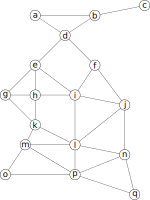
\includegraphics[width=0.7\columnwidth]{8/graph.pdf}
    \caption{{\color{gray} The graph depicting the connectedness of the Wireless Sensor Network under consideration.}}
    \label{fig:8}
\end{figure}

\renewcommand{\labelenumi}{(\alph{enumi})}
\begin{enumerate}
  \item {\color{gray} Suppose 9 frequency channels are available, can the chosen communication protocol be used in the shown network?}
  \item {\color{gray} Determine the minimum number of channels required to be able to use the chosen communication protocol in the shown network.}
  \item {\color{gray} Suppose a different communication protocol requires unique frequency channels in each 3-hop neighborhood instead and 11 channels are available. Determine if this other communication protocol can be used in the shown network. (This means for all nodes $i$, no nodes $j$, $k$ and $l$ with edges $i$-$j$, $j$-$k$ and $k$-$l$ may exist where the channel of $j$, $k$ or $l$ is equal to the channel of $i$.)}
\end{enumerate}

In order to solve this problem an SMT implementation is made which will be detailed below. For each set of two nodes $x$ and $y$ the variables $hop\_1\_x\_y$ and $hop\_1\_y\_x$ are defined. For each pair of nodes that are connected by an edge the constraint is added that the corresponding variables are true, for each pair of nodes that do not share an edge the requirement is added that the corresponding variables are false. This process defines all edges and therefore 1-hop neighbors in the network.

In order to define the $i$-hop neighbors the constraints $hop\_i\_x\_y \implies hop\_{i+1}\_x\_y$ and $hop\_i\_x\_y \vee hop\_1\_y\_z \implies hop\_{i+1}\_x\_z$ are implemented for all possible permutations of the nodes $x$, $y$ and $z$. This process defines the $i$-hop neighbors from the $i-1$-hop neighbors and one extra edge.

\begin{enumerate}
  \item The requirement that the frequency channel should be unique in each 2-hop neighborhood can be expressed by the constraints $hop\_2\_x\_y \implies chan\_x \neq chan\_y$ for all permutations of the nodes $x$ and $y$, while the requirement that only 9 channels are available can be expressed by the constraints $0 \leq chan\_x \leq 8$. Generating the conjunction of all constraints by the Python script listed in \Cref{app:4_gen.py} yields the SMT file listed in \Cref{app:4_a_in}. Running Z3 on this file shows the satisfying assignment listed in \Cref{app:4_a_out} from which it can be concluded that the following channel assignment is a valid assignment:
  \begin{table}[]
    \begin{tabular}{ll|ll}
      Node & Channel & Node & Channel \\ \hline
      A    & 3       & J    & 1       \\
      B    & 6       & K    & 0       \\
      C    & 5       & L    & 3       \\
      D    & 0       & M    & 2       \\
      E    & 5       & N    & 5       \\
      F    & 4       & O    & 4       \\
      G    & 1       & P    & 7       \\
      H    & 7       & Q    & 6       \\
      I    & 8       &      &        
   \end{tabular}
  \end{table}
  This shows that it is indeed possible to use the chosen protocol in the network with 9 channels available.
  \item Changing the requirements regarding the number of channels to $0 \leq chan\_x \leq 6$ and $0 \leq chan\_x \leq 5$ for all nodes $x$ yields the SMT files listed in \Cref{app:4_b1_in} and \Cref{app:4_b2_in} respectively. Running Z3 on these files produces the outputs listed in \Cref{app:4_b1_out} and \Cref{app:4_b2_out} respectively. The fact that the constraints with $0 \leq chan\_x \leq 5$ are unsatisfiable means that there is no way to assign the frequency channels if only 6 channels are available, while for 7 available channels the following assignment is found:
  \begin{table}[]
    \begin{tabular}{ll|ll}
      Node & Channel & Node & Channel \\ \hline
      A    & 1       & J    & 5       \\
      B    & 0       & K    & 4       \\
      C    & 4       & L    & 1       \\
      D    & 2       & M    & 2       \\
      E    & 6       & N    & 6       \\
      F    & 4       & O    & 5       \\
      G    & 5       & P    & 3       \\
      H    & 3       & Q    & 4       \\
      I    & 0       &      &        
   \end{tabular}
  \end{table}
  From this it can be concluded that the minimum number of available channels required is 7.
  \item The constraints concerning the number of available channels can be changed to $0 \leq chan\_x \leq 10$ for all nodes $x$, while the constraints that specify unique channels in a 3-hop neighborhood can be represented by $hop\_3\_x\_y \implies chan\_x \neq chan\_y$ for all permutations of nodes $x$ and $y$. This results in the SMT file listed in \Cref{app:4_c_in}, while running Z3 on this file generates the output listed in \Cref{app:4_c_out}. This output shows that the following channel assignment satisfies all requirements:
  \begin{table}[]
    \begin{tabular}{ll|ll}
      Node & Channel & Node & Channel \\ \hline
      A    & 6       & J    & 4       \\
      B    & 3       & K    & 3       \\
      C    & 4       & L    & 6       \\
      D    & 5       & M    & 5       \\
      E    & 7       & N    & 8       \\
      F    & 0       & O    & 7       \\
      G    & 9       & P    & 10      \\
      H    & 2       & Q    & 9       \\
      I    & 1       &      &        
   \end{tabular}
  \end{table}
  From this it can be concluded that the alternative communication protocol can be used in the network if 11 channels are available.
\end{enumerate}
